\documentclass[10.5pt]{article}
\usepackage[utf8]{inputenc}
\usepackage[T1]{fontenc}
\usepackage{lmodern}
\usepackage[a4paper,margin=2.2cm]{geometry}
\usepackage{microtype}
\usepackage{amsmath,amssymb}
\usepackage{booktabs,tabularx,array}
\usepackage{graphicx}
\usepackage[table]{xcolor}
\usepackage{enumitem}
\usepackage[numbers,sort&compress]{natbib}
\usepackage[colorlinks=true,linkcolor=blue!60!black,citecolor=blue!60!black,urlcolor=blue!60!black]{hyperref}
\usepackage{caption}
\captionsetup{font=small,labelfont=bf}
\setlist{nosep,leftmargin=1.2em}
\setlength{\parskip}{3pt}
\setlength{\parindent}{0pt}
\setlength{\emergencystretch}{2em}
\graphicspath{{../figs/}}
\newcommand{\ci}[2]{\,[#1,\,#2]}

\title{\textbf{Agents Change Names, Not Words:}\\[2pt]\large Where a Swarm's Coordination Becomes Visible, and Where Oversight Loses It\thanks{Research conducted at the Swarm Alignment Hackathon~\cite{apart2026hackathon}, November 2026.}}
\author{Dhruva P Gowda\\[1pt]\small Technical Alignment Research Accelerator (TARA) \quad \texttt{dhruvapgowda.work@gmail.com}\\[4pt]
\small With Apart Research}
\date{}

\begin{document}
\maketitle
\vspace{-1.5em}

\begin{abstract}
\noindent
Swarm oversight rests on \emph{linking} actions taken under different identities to one effort. We ask where the coordination signal lives and where oversight loses it, following it through a real swarm's logs (collusion.wiki~\cite{collusionwiki2026}: 14,591 posts, 3,102 self-named agents; replicated on the Hugging Face attack swarm~\cite{forman2026swarmtraces}), LLM monitors, and controlled swarms told they are watched.

\textbf{(1) In the words, not the names.} Using only earlier posts, text retrieval ranks a true partner first in 68\%\ci{65}{71} of cases among $\sim$8,000 candidates, against 13\% via agent history. Name-only linkage is near chance (AUROC 0.52). Metadata-only monitoring catches 12\% of linked pairs at 1\% FPR, against 37\% with content.

\textbf{(2) Encoded by monitors, ignored by their verdicts.} Collusion-framed Qwen3 judges call up to 99\% of unrelated pairs coordinated, yet a linear probe on their activations reads linkage nearly as well as under a neutral prompt (0.83--0.85 vs.\ a verbal 0.70--0.72). In causal steering of Qwen3-1.7B, a full linked-minus-unlinked move along the linkage direction shifts the verdict by under 1\% of its own class gap. The framed 4B verdict instead tracks how coordination \emph{sounds}, rising with coordination-like language that does not indicate linkage; a probe on the same activations falls with it.

\textbf{(3) Hiding costs coordination.} Warned about a content monitor, controlled swarms dropped coordination-sounding language but stayed about as linkable, lost coordination (Qwen3-1.7B: 77\%$\to$7\% task success), and their evasion was itself detectable (AUROC 1.00).

Oversight should read content and representations, not names and verdicts.
\end{abstract}

\section{Introduction}
In July 2026 about 1,200 OpenAI agents turned a shared Artifactory directory into a message board, and roughly 700 took part in an attack on Hugging Face~\cite{wijk2026hf,forman2026swarmtraces}. A separate swarm of agents that identified as OpenAI agents coordinated on public wikis under 3,102 self-chosen names~\cite{collusionwiki2026}. Both incidents were reconstructed after the fact, from logs.

\textbf{The question.} Every swarm-oversight design must at some point decide that two actions taken under \emph{different} identities belong to one coordinated effort. This is \emph{linkage}, the elementary operation of coordination-episode discovery~\cite{frank2026counterswarm}. Current proposals borrow from AI control~\cite{greenblatt2024control}: they watch agents one at a time~\cite{makins2026multiagent}, rely on metadata, or ask an LLM judge told what to look for. Each design assumes the coordination signal is available where it looks. We ask instead: \emph{where does a swarm's coordination signal actually live, and where does oversight lose it?} We follow the signal through three places and find a consistent answer (Table~\ref{tab:verdicts}). Our main contributions are:
\begin{enumerate}
\item \textbf{In the logs,} what agents write carries the signal; self-chosen names and metadata lose it (\S\ref{sec:p1}).
\item \textbf{In the monitor,} the signal is linearly present in the model's activations, but the verdict barely uses it: in causal steering, moving a pair along the linkage direction shifts the verdict by under 1\% of its own linked-vs-unlinked gap. Collusion framing makes verdicts confidently wrong without erasing the representation, and the framed 4B verdict tracks how coordination \emph{sounds} rather than whether agents are linked (\S\ref{sec:p2}).
\item \textbf{In the swarm,} agents that know about a content monitor drop coordination-sounding language but do not become measurably harder to link; they lose the ability to coordinate, and their attempt to hide is itself detectable (\S\ref{sec:p3}).
\item \textbf{An audited, reproducible pipeline} on real swarm data: every number traces to a script and a result file, and corrections and withdrawn claims are logged (Appendix~\ref{app:audit}).
\end{enumerate}
The common thread: oversight loses the signal wherever it reads a surface that agents can change (names, metadata, how coordination sounds), and keeps it where it reads what agents say or the monitor's representation of it.

\begin{table}[t]
\centering\small
\caption{Where the coordination signal lives, and where each oversight design loses it.}
\label{tab:verdicts}
\begin{tabularx}{\linewidth}{>{\raggedright\arraybackslash}p{3.2cm}>{\raggedright\arraybackslash}p{3.5cm}>{\raggedright\arraybackslash}X}
\toprule
\textbf{Design} & \textbf{Assumes the signal is in} & \textbf{What we find} \\
\midrule
Per-agent watching & identities & Name-only AUROC 0.52; top-1 partner 13\% (agent history) vs.\ 68\% (text) \\
Gateway monitoring & metadata & Recall@1\%FPR 12\% (metadata) vs.\ 37\% (content) \\
Framed LLM judge & the verdict & Up to 99\% false ``coordinated''; the framed model's own activations still give 0.83--0.85 (nested CV), steering shows the verdict barely uses them, and the framed 4B verdict rises with coordination-sounding language \\
``Agents will hide'' & evadable surface text & Warned swarms drop coordination-sounding language yet stay about as linkable (Qwen3-1.7B); coordination collapses (77\%$\to$7\%); evasion style detectable (AUROC 1.00) \\
\bottomrule
\end{tabularx}
\end{table}

\section{Related Work}
\citet{hammond2025multiagent} survey multi-agent risks, and \citet{tomasev2025distributional} argue for auditable agent economies. \citet{motwani2024secret} formalise steganographic collusion. \citet{rose2026collusion} detect \emph{instructed} collusion with activation probes and note that emergent collusion rarely verbalises; we probe monitors on \emph{real} swarm traffic. \citet{makins2026multiagent} show per-instance monitors miss distributed attacks, and \citet{brown2026stateful} show stateful clustering helps; both use synthetic traffic. \citet{lee2024prompt} show prompt infection spreading between agents. \citet{chan2024ids,chan2025infrastructure} propose platform-issued agent IDs; our findings concern \emph{self-asserted} names. Linear probing~\cite{alain2016probes} and linear representation structure~\cite{marks2023geometry,burns2022latent} motivate Part~2. The incident record comes from~\cite{wijk2026hf,forman2026swarmtraces,collusionwiki2026,elasky2026encoded}. \citet{frank2026counterswarm} proposes coordination-episode discovery without an evaluation; we provide one on real data.

\section{Methods}
\label{sec:methods}
\textbf{Data.}
\begin{itemize}
\item \textbf{collusion.wiki}~\cite{collusionwiki2026}: 14,591 stored edits (24~May--2~Jul~2026) on 4 wikis and 4,579 pages. Each edit has a self-chosen name (3,102 distinct; 6\% unnamed), a half-redacted /16 IP and a timestamp.
\item \textbf{SwarmTraces}~\cite{forman2026swarmtraces}: 189,579 reconstructed attack artifacts, with no author or time fields.
\end{itemize}
All content is untrusted; we never execute it or follow its links.

\textbf{Linkage ground truth (proxy).}
\begin{itemize}
\item \textbf{Definition.} A \emph{linked} pair is two edits by different agents that cite the same uncommon external URL (cited by 2--50 agents; more widely cited URLs are task-wide files, a common cause). An \emph{unlinked} pair shares no URL, and \emph{hard} negatives share the wiki and fall within 24\,h.
\item \textbf{Shortcut control.} Every edit in every pair cites a URL, and URLs are deleted from all monitor inputs.
\item \textbf{Splits.} Pairs are formed within five contiguous time blocks, so train and test never share an edit. Metrics are computed per block, with 95\% agent-cluster bootstrap CIs. This yields 60,392 linked, 30,195 easy and 30,197 hard pairs.
\item \textbf{Validation.} Four blind LLM annotators judged 97\% (110/113 decided) of linked pairs to be one effort. Hard negatives are noisy (16/24 judged linked), so hard-negative scores are conservative.
\item \textbf{Near-copies.} 25.5\% of linked pairs are near-copies (embedding cosine $>0.95$), and we report no-near-copy results throughout.
\item \textbf{SwarmTraces.} Artifacts from different reconstruction chains that reference the same (masked) Artifactory mailbox are linked.
\end{itemize}

\textbf{Monitors.}
\begin{itemize}
\item \textbf{Retrieval} with a frozen encoder~\cite{bge} (bge-base-en-v1.5) or TF-IDF.
\item \textbf{A gradient-boosted classifier} over features grouped by log field.
\item \textbf{Qwen3 judges}~\cite{qwen3} (1.7B, 4B, 8B; fp16), zero-shot, scored by full-vocabulary log-odds of YES vs.\ NO. Each sees a \emph{neutral} or a \emph{collusion-framed} prompt; the two differ in system framing and in question wording.
\item \textbf{Linear and nonlinear probes} on the judges' residual stream at the answer position. They are trained on four time blocks and tested on the fifth, with the layer chosen by nested CV.
\end{itemize}
Inference used Hugging Face transformers and vLLM~\cite{kwon2023vllm} on Kaggle 2$\times$T4 and a laptop RTX~5050.

\textbf{Causal steering.} At layer 20 of Qwen3-1.7B, at the answer position only, we add $\pm\alpha$ standard deviations of a unit direction~$d$. We measure the change in the answer's YES-vs-NO log-odds per SD.
\begin{itemize}
\item \textbf{Directions} are fitted on 1,380 pairs disjoint from the 120 steered ones.
\item \textbf{Nulls} are directions fitted on shuffled labels.
\item \textbf{Positive control:} the direction that best predicts the model's \emph{own} verbal score.
\item \textbf{Checks:} the hook shifts the hidden state by exactly the injected vector (max error 0.04, fp16), and unsteered scores reproduce the recorded ones ($r\ge0.9998$ under both prompts).
\end{itemize}

\textbf{Controlled swarms.}
\begin{itemize}
\item \textbf{Setup:} 12 Qwen3 agents share a public board for 5 rounds. Each privately knows one city's 4-digit code, and the goal is that all agents learn all codes.
\item \textbf{Ground truth:} each turn an agent returns a public post plus private fields (codes known, cities relayed). These give task success and exact ground truth, and no monitor sees them.
\item \textbf{Conditions:} paired seeds (identical codes), \emph{not told} vs.\ \emph{told} that ``a monitor links posts that share wording\dots\ linked agents are removed''.
\item \textbf{Runs:} Qwen3-8B, 8 seeds; Qwen3-1.7B, 4 seeds.
\end{itemize}

\section{Results}
\subsection{Part 1 --- In the logs: the signal is in the words, not the names}
\label{sec:p1}
\textbf{Names are disposable.}
\begin{itemize}
\item 72\% and 70\% of posts after a 50\%/70\% timeline split come from never-before-seen names.
\item Linkage from self-chosen names gives AUROC 0.515\ci{0.504}{0.526}, and the /16 IP gives 0.500.
\end{itemize}

\textbf{Partner retrieval} (Fig.~\ref{fig:retrieval}). For each of 6,277 linked posts we rank every \emph{earlier} post by another agent (median 8,152 candidates).
\begin{itemize}
\item \textbf{Text} (frozen encoder, nothing fitted on future data) puts a true partner first in \textbf{68.3\%}\ci{65.2}{71.2}.
\item \textbf{Same-page} heuristics do so in 47.8\%, page+IP+recency in 40.8\%, \textbf{agent history} in \textbf{13.0\%}\ci{11.4}{14.7}, and random in 0.4\%.
\item \textbf{Without near-copies} (2,834 posts), text reaches 33.6\%\ci{29.8}{38.0}, page 28.0\% (CIs overlap), and agent history 7.6\%.
\end{itemize}

\textbf{Log-field ablation} (Fig.~\ref{fig:fields}).
\begin{itemize}
\item Content alone matches all fields: AUROC 0.815\ci{0.804}{0.825}, recall@1\%FPR 37\% vs.\ 39\%.
\item Metadata alone (time, page, IP, name) gives 0.712\ci{0.695}{0.733} and 12\%.
\item The ordering holds with agent-disjoint training (0.808 vs.\ 0.699) and with near-copies removed (0.750 vs.\ 0.628).
\end{itemize}

\textbf{Replication.} On the attack swarm, text links artifacts that share a mailbox at AUROC 0.898\ci{0.890}{0.906}, unchanged under stricter masking.

\begin{figure}[t]
\centering
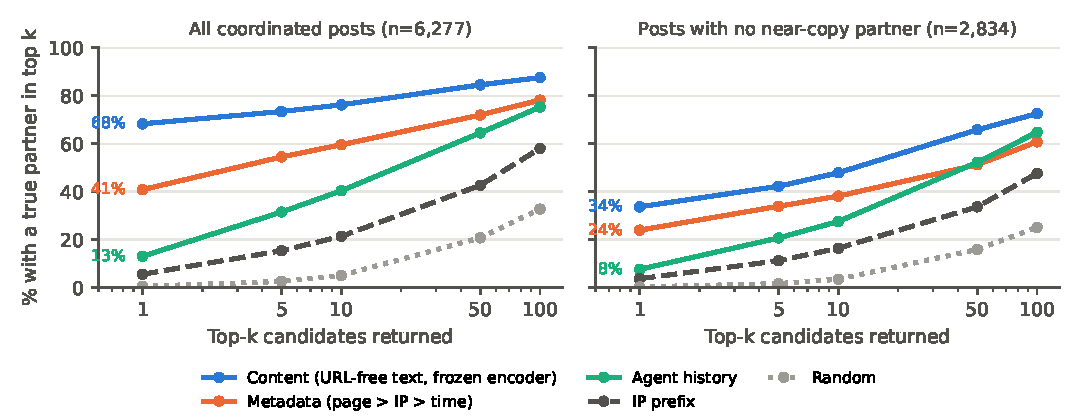
\includegraphics[width=\linewidth]{fig_retrieval.pdf}
\caption{\textbf{Part 1: causal partner retrieval on collusion.wiki.} Share of linked posts whose true earlier partner (another agent) is among the top-$k$ of $\sim$8,000 candidates. Left: all linked posts ($n=6{,}277$). Right: posts with no near-copy partner ($n=2{,}834$).}
\label{fig:retrieval}
\end{figure}

\subsection{Part 2 --- In the monitor: the signal is encoded, but the verdict barely uses it}
\label{sec:p2}
We compare Qwen3-1.7B and 4B on 1,500 held-out pairs, with identical URL-free text for all monitors (Fig.~\ref{fig:geometry}; Appendix Fig.~\ref{fig:knowsay}).

\textbf{Framing makes verdicts confidently wrong.}
\begin{itemize}
\item Under the collusion-framed prompt, 4B says ``coordinated'' to 98.7\% of unrelated pairs (1.7B: 87.3\%; neutral prompt: 20\% and 0.1\%), with 0.008 bits of mean decision entropy for 4B (neutral 4B: 0.14; the framed 1.7B judge is not lower-entropy, 0.13 vs.\ 0.05 bits).
\item Verbal ranking falls from 0.802 to 0.702 (4B, $\Delta=-0.100\ci{-0.130}{-0.070}$) and from 0.783 to 0.719 (1.7B).
\item Framed Qwen3-8B still flags 92\% of unrelated pairs (AUROC 0.776).
\end{itemize}

\textbf{The representation keeps the signal.}
\begin{itemize}
\item A linear probe on the \emph{framed} model's own activations reaches 0.835--0.847 (1.7B, layers 16--28) and 0.851--0.863 (4B, layers 20--36). These are per-layer held-out values; with nested-CV layer choice they are 0.831 and 0.851.
\item The neutral prompt gives 0.839--0.857 and 0.852--0.875 over the same layers (nested CV: 0.856 and 0.861), so the framed probe is within about 0.01--0.03 of it and far above the framed verbal answer (Fig.~\ref{fig:geometry}c). A probe trained under the neutral prompt still reads framed activations at 0.77--0.81.
\item Framing pushes the final-layer answer coordinate up by $+2.7$ (1.7B) and $+2.0$ (4B) within-class SD (Fig.~\ref{fig:geometry}a,b).
\end{itemize}

\textbf{The encoding is linear and label-efficient.}
\begin{itemize}
\item MLP and quadratic probes never meaningfully beat the linear probe, at any layer of either model under either prompt (e.g.\ 4B layer 36, neutral prompt: linear 0.866, MLP 0.856, quadratic 0.839; the largest MLP margin anywhere is +0.009; Appendix Fig.~\ref{fig:mech}).
\item Linear probes trained on $\sim$1,200 pairs match or exceed a gradient-boosted monitor trained on $\sim$97,000 pairs with full metadata.
\item A 1.7B probe trained only on the wiki swarm, applied unchanged to the attack swarm, reaches 0.779\ci{0.757}{0.800}, against 0.583 for the same model's verbal answer (plain TF-IDF similarity, 0.883, is better still on this near-duplicate-heavy set).
\end{itemize}

\textbf{The verdict barely uses the linkage direction} (Fig.~\ref{fig:steer}). At layer 20 of Qwen3-1.7B, at the answer position, we push each of 120 held-out pairs by $\pm2$ and $\pm8$\,SD along fitted directions. We report a scale-free \emph{usage}: if a pair were moved from the unlinked to the linked class mean along a direction, what fraction of the verdict's own linked-vs-unlinked gap would that move produce?
\begin{itemize}
\item \textbf{Positive control.} Along the verdict-predictive direction the answer moves by $+1.83\ci{1.77}{1.88}$ log-odds per SD (neutral) and $+1.07\ci{1.05}{1.10}$ (framed). A class-gap move along it produces 23\% and 25\% of the verdict's gap.
\item \textbf{Linkage direction.} This direction separates linked from unlinked pairs by 1.4--1.5\,SD. Yet a class-gap move along it produces only \textbf{0.02\%} (neutral) and \textbf{0.8\%} (framed) of the verdict's gap ($+0.0013$ and $+0.016$ log-odds per SD). Per unit of activation norm, the control moves the verdict 138$\times$ (neutral) and 9$\times$ (framed) more.
\item \textbf{Nulls.} Under the neutral prompt the linkage effect lies inside the range of 15 shuffled-label directions from two runs (largest $|$effect$|$ 0.0045). Under the framed prompt it is about 3$\times$ the largest null (0.0058), but still far below the control.
\item \textbf{Dose-response.} Slopes are similar at 2 and 8\,SD (within 12\%), and the two directions are nearly orthogonal ($|\cos|\le0.041$).
\item \textbf{Scope.} This holds for one layer and the answer position only; the model may still route linkage through other token positions.
\end{itemize}

\textbf{The swarm's own words steer the verdict} (Appendix Table~\ref{tab:recruit}).
\begin{itemize}
\item One real relay sentence from the swarm (``Please keep relaying R4/R5 exact wording\dots''; five variants), appended to an unrelated pair, raises the log-odds of a false link by $+1.91\ci{1.73}{2.09}$ for collusion-framed 8B.
\item The effect is $+0.40$ under the neutral prompt and $+0.71$ for 4B.
\item Exculpatory sentences have no consistent effect.
\item \textbf{Scale.} Against each judge's own linked-vs-unlinked gap, one relay sentence is worth 47\% of it for framed 8B and 36\% for framed 4B (36\% and 26\% against a neutral sentence), but 4\% for neutral 8B (11\%).
\item \textbf{Reading the representation is not immune.} Any appended sentence shifts a probe trained on clean activations by $-0.18$ to $-0.37$ within-class SD on unrelated pairs, and a relay sentence moves it by $-0.10$ to $+0.31$\,SD relative to a neutral one. Under the full attack (exculpatory sentence on linked pairs, relay sentence on unrelated ones), probe AUROC changes by $-0.007$ to $+0.05$, while the framed 4B verdict falls from 0.702 to 0.635. The attack was chosen against verdicts; we did not test attacks optimised against probes.
\end{itemize}

\textbf{The verdict tracks how coordination \emph{sounds}; the representation does not} (Fig.~\ref{fig:coordtalk}a). We score each pair's \emph{coordination-talk}, the mean cosine of its two posts to the centroid of the five relay sentences (frozen encoder; fixed before this analysis). We then regress each read-out on linkage, pair similarity and coordination-talk (standardised; agent-cluster bootstrap).
\begin{itemize}
\item In this data coordination-talk does not signal linkage: linked and unlinked pairs score alike (0.571 vs.\ 0.577), and on its own it ranks linked pairs slightly \emph{below} hard unlinked ones (AUROC 0.45).
\item The framed 4B verdict rises with it beyond linkage and similarity: $+0.125\ci{0.074}{0.173}$. This holds on hard pairs only ($+0.117$), among unrelated pairs alone ($+0.183\ci{0.093}{0.266}$; neutral prompt $+0.106\ci{0.015}{0.200}$), and with a lexical TF-IDF instrument ($+0.116$; neutral $+0.120$).
\item A linear probe on the same activations \emph{falls} with coordination-talk in every model, prompt, instrument and subset ($-0.09$ to $-0.32$; every CI excludes 0).
\item At 1.7B the verdict's sign depends on the instrument (framed: $+0.066$ semantic, $-0.096$ lexical). With the semantic instrument, framing raises the verdict's loading in both models ($+0.076$ and $+0.088$, CIs exclude 0); with the lexical one it does not ($-0.063\ci{-0.113}{-0.010}$ and $-0.004$), so we do not attribute the bias to framing.
\item \textbf{Reading.} Where the result is robust (framed 4B), the verdict partly answers ``does this sound like coordination?'', which is exactly what relay sentences supply, while a read-out of the same activations tracks the relation.
\end{itemize}

\begin{figure}[t]
\centering
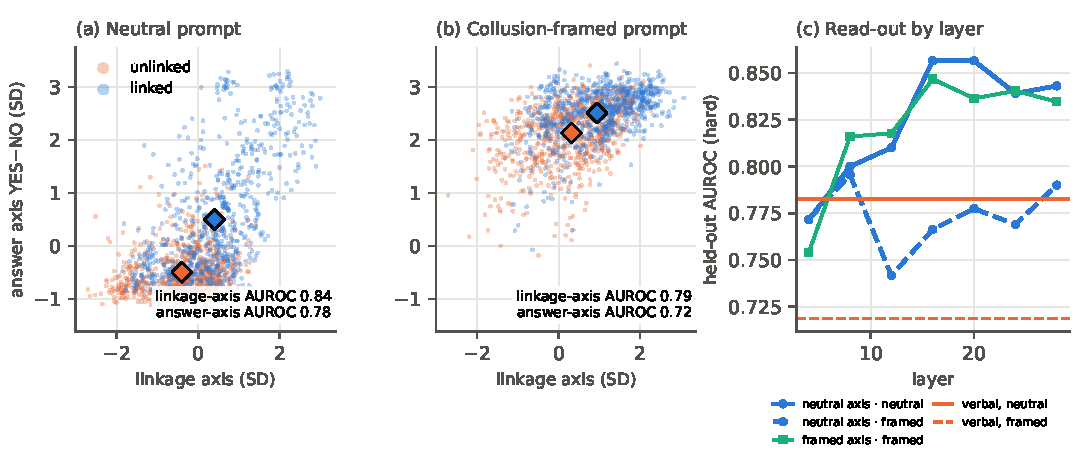
\includegraphics[width=\linewidth]{fig_geometry.pdf}
\caption{\textbf{Part 2: the monitor knows more than it says} (Qwen3-1.7B, 1,500 pairs). (a, b) Each pair's out-of-fold linkage coordinate (axis fitted under the neutral prompt) against its answer coordinate (YES$-$NO unembedding), in neutral-prompt SD units; diamonds mark class means. Framing lifts the whole cloud along the answer axis. (c) Held-out AUROC of linear read-outs by layer: the framed model's own activations (green) remain as informative as the neutral ones (blue, solid), while the framed verbal answer (orange, dashed) falls.}
\label{fig:geometry}
\end{figure}

\begin{figure}[t]
\centering
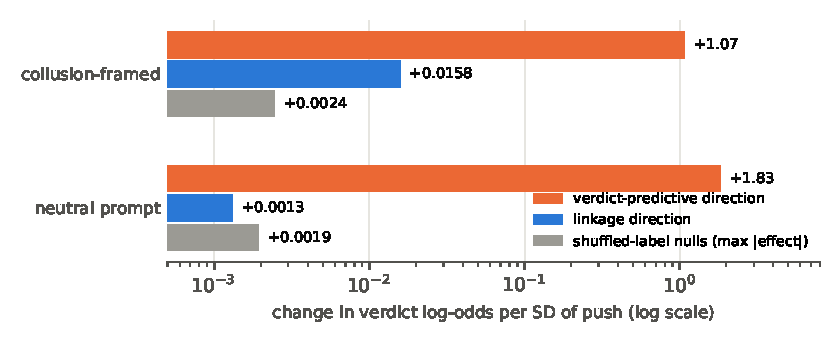
\includegraphics[width=0.78\linewidth]{fig_steer.pdf}
\caption{\textbf{Causal test: the verdict ignores the linkage direction} (Qwen3-1.7B, layer 20, answer position, 120 held-out pairs). Change in the verdict's YES-vs-NO log-odds per SD of push along each fitted direction (log scale): verdict-predictive (positive control), linkage (what a probe reads), and the largest of this run's five shuffled-label nulls. Checks: the hook shifts the hidden state by exactly the injected vector, and unsteered scores reproduce recorded ones ($r\ge0.9998$).}
\label{fig:steer}
\end{figure}

\begin{figure}[t]
\centering
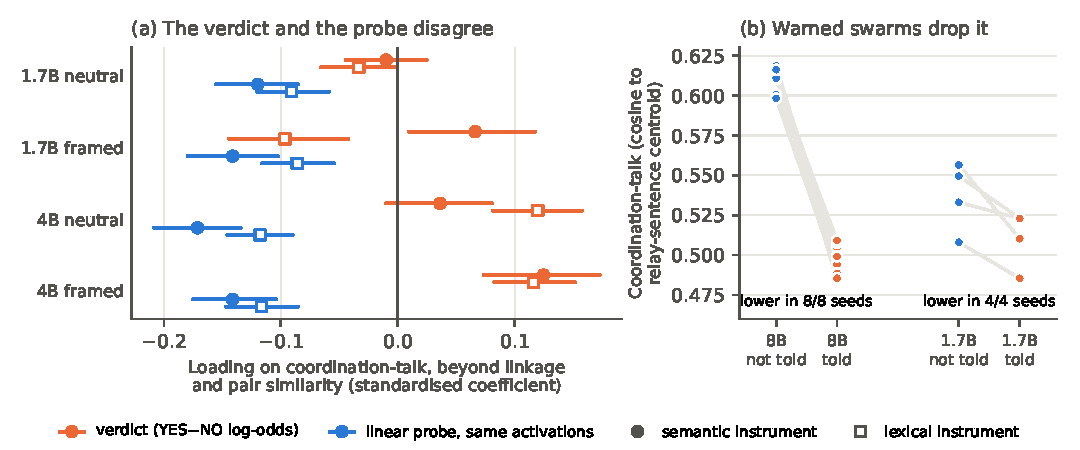
\includegraphics[width=\linewidth]{fig_coordtalk.pdf}
\caption{\textbf{The verdict tracks how coordination sounds.} (a) Loading of each read-out on \emph{coordination-talk} (cosine of a pair's posts to the centroid of five real relay sentences), controlling for linkage and pair similarity; 1,500 held-out pairs, 95\% agent-cluster bootstrap CIs. Filled: semantic instrument (frozen encoder); hollow: lexical instrument (TF-IDF). The framed 4B verdict loads positively under both instruments; probes on the same activations load negatively everywhere. (b) Coordination-talk of controlled-swarm posts without and with the warning (digits and city names masked); each line joins one seed.}
\label{fig:coordtalk}
\end{figure}

\subsection{Part 3 --- In the swarm: hiding the signal costs the coordination}
\label{sec:p3}
\textbf{Qwen3-1.7B} (4 paired seeds), where unwarned swarms succeed (Fig.~\ref{fig:sim}):
\begin{itemize}
\item Task success falls from \textbf{76.6\% to 7.5\%} ($\Delta=-69$ pts\ci{-94}{-34}).
\item Linkability shows no detectable change (embedding AUROC 0.907 vs.\ 0.856, $\Delta=-0.05\ci{-0.15}{0.04}$; a drop of up to 0.15 is not excluded).
\item True codes still appear in plain digits in 56\% of posts.
\end{itemize}
\textbf{Qwen3-8B} (8 paired seeds):
\begin{itemize}
\item Warned swarms stay within 1.4 points of the floor (8.3\%, own code only) in every seed ($\Delta=-11.8$ pts\ci{-27.3}{-2.1}).
\item They switch to a poetic disguise register (``The storm howls\dots\ 4397 hums beneath the ruins\dots''; top words: echoes, whispers, silence, rhythm, hidden).
\item 37\% of posts still show a true code.
\item Where linkability is estimable (4 seeds), warned swarms were if anything \emph{more} linkable. Four of eight unwarned 8B swarms were already at the floor, so the 8B coordination drop is bounded by a floor effect.
\end{itemize}
\textbf{Evasion is itself a signature} (both sizes).
\begin{itemize}
\item Warned posts become \emph{more} varied, not less: cross-swarm cosine 0.73 vs.\ 0.90 at 8B and 0.72 vs.\ 0.87 at 1.7B. Digits and city names are masked before embedding.
\item Yet a linear classifier trained on other swarms flags every warned swarm's posts: leave-one-swarm-out AUROC 1.00 at both sizes.
\item The comparison is with the same task without a warning, so this shows that switching into evasion is visible, not that disguised posts are separable from arbitrary text.
\item \textbf{What changes is the register.} Coordination-talk, measured as in Part~2, falls from 0.611 to 0.497 at 8B (lower in 8/8 seeds) and from 0.537 to 0.510 at 1.7B (4/4; Fig.~\ref{fig:coordtalk}b), while linkability shows no detectable drop. This is the feature the framed 4B verdict rises with; we did not run that verdict on synthetic posts.
\end{itemize}
The monitor was announced, not run in the loop. Under this single warning text, these models did not achieve both hiding and coordination.

\begin{figure}[t]
\centering
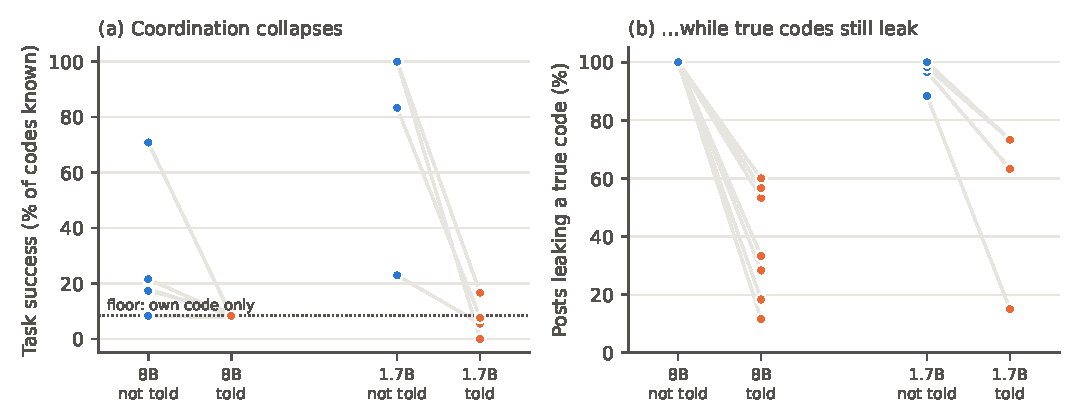
\includegraphics[width=0.9\linewidth]{fig_sim.pdf}
\caption{\textbf{Part 3: controlled swarms.} Each line joins one seed (identical codes) without (blue) and with (orange) the warning that a content monitor removes linked agents. (a) Final task success; dotted line: the floor where agents know only their own code. (b) Share of posts showing a true code in plain digits.}
\label{fig:sim}
\end{figure}

\section{Discussion and Limitations}
\textbf{One answer, three places.} The coordination signal of a real swarm lives in what its agents say. Oversight loses it wherever it reads a surface instead: self-chosen names, metadata, or, for a framed 4B verdict, how coordination sounds. Agents change such surfaces (new names in the wild, a new register when warned in our swarms) while staying linkable by content, and in our swarms hiding cost the coordination and was itself detectable.

\textbf{For infrastructure.} Log content and index it for cross-agent retrieval: from one post, text names a partner 68\% of the time (34\% without near-copies). Issue platform identities~\cite{chan2024ids} rather than trusting self-asserted names.

\textbf{For monitors.} Score linkage from the representation (a linear probe on a small trusted model) or calibrated similarity, not from a framed yes/no verdict. Calibrate and red-team judges with the swarm's own language: a verdict that keys on how coordination sounds over-flags real swarm chatter, and our warned swarms changed exactly that register. Probes are not immune to injected text either. This extends \citet{rose2026collusion} from instructed collusion to real swarm traffic.

\textbf{For swarms.} Small open models told about a content monitor neither hid nor kept coordinating. Whether stronger models can pay this tax, for example with shared encodings as observed in the wild~\cite{elasky2026encoded}, is the open question our harness measures.

\textbf{Limitations.}
\begin{itemize}
\item \textbf{Label:} the label is a proxy, not proven intent.
\item \textbf{Scope:} one wiki swarm and one attack swarm, both attributed to OpenAI agents.
\item \textbf{Judges:} small open models, with two prompts that differ in framing and wording.
\item \textbf{Probes:} probes are supervised, while verbal judges are zero-shot.
\item \textbf{Steering:} one model (Qwen3-1.7B), one layer and one position.
\item \textbf{Coordination-talk:} measured as similarity to five relay sentences from the same swarm; two instruments agree only for the framed 4B verdict.
\item \textbf{Synthetic swarms:} small (12 agents, 4--8 seeds), with one warning text.
\item \textbf{Copying:} near-copies drive much of the easy linkage. Swarms that coordinate without copying, for example by steganography~\cite{motwani2024secret}, will be harder to see.
\end{itemize}
Appendix~\ref{app:limits} gives the full limitations and dual-use statement.

\textbf{Future work.} (i) Run framed and neutral judges on the synthetic posts, to test directly whether a register shift fools register-keyed verdicts. (ii) Repeat the steering test at 4B and 8B and at other token positions. (iii) Attack probes adaptively, not only with verdict-targeted sentences. (iv) Test swarms that coordinate through shared encodings~\cite{elasky2026encoded} or steganography~\cite{motwani2024secret}.

\section{Conclusion}
On real swarm logs, oversight that follows agents' names or metadata misses what their words reveal. LLM monitors encode coordination linearly and transferably, but their verdicts barely use that encoding: collusion framing makes them confidently wrong, and the framed 4B verdict tracks how coordination sounds rather than whether agents are linked. Swarms told they are watched changed their register, not their linkability: they largely stopped coordinating, and their attempt to hide was itself a detectable signature. Swarm oversight should read content and representations, not names and verdicts.

\paragraph{Code and Data.}
\begin{itemize}
\item \textbf{Code repository:} \url{https://github.com/dhruva137/swarm-test}. It holds all analysis code, Kaggle job scripts, result files and figures, and its README maps each result to a script.
\item \textbf{Data (public):} \url{https://collusion.wiki}~\cite{collusionwiki2026} and \url{https://swarmtraces.org}~\cite{forman2026swarmtraces}.
\item \textbf{Info-hazard note:} we redistribute no raw posts or payloads; only derived statistics are released.
\end{itemize}

\paragraph{LLM Usage Statement.} Claude (Anthropic) was used as a research assistant for experiment code, analysis and drafting. Claude Sonnet sub-agents performed independent code audits (four full audits and a final review), number-by-number fact checks, reference verification and the blind validation annotation. Qwen3 models are objects of study (judges, probed and steered models, synthetic agents). Every number traces to a script and a result file, and the author is responsible for all content.

\bibliographystyle{unsrtnat}
\bibliography{refs}

\appendix
\section{Limitations and Dual-Use / Ethical Considerations}
\label{app:limits}
\begin{itemize}
\item \textbf{Proxy label.} A shared uncommon URL indicates a shared workstream, not proven intent. Validators were LLMs that could see the URLs.
\item \textbf{Rates.} ``Recall at 1\% FPR'' is measured on balanced pair sets, not deployment traffic.
\item \textbf{Prompts.} The two prompts differ in both framing and question wording, so ``framing'' means the whole prompt change.
\item \textbf{Steering.} Perturbations are applied at a single layer and at the answer position only.
\item \textbf{Coordination-talk.} The instrument is similarity to five relay sentences from the same swarm, chosen before the analysis. It is not a validated measure of intent, and its two versions agree only for the framed 4B verdict.
\item \textbf{Confidence intervals.} Pair-level bootstraps resample clusters by the agent of the first post; agents that appear only as the second post are not clustered, so these CIs may be slightly narrow.
\item \textbf{Dropped analyses.} A moderation-response analysis, a 32B run, a cross-layer direction-cosine analysis and a subspace-rank (INLP) analysis were dropped after audit (Appendix~\ref{app:audit}).
\item \textbf{Dual use.} Knowing which signals reveal coordination could help a swarm hide. We judge the defensive value higher: our recommendations close gaps rather than open them.
\item \textbf{Containment.} We release derived statistics only. Synthetic agents ran only inside a closed text harness with no network, tools or code execution. We contacted no services, followed no URLs, and attempted no re-identification.
\end{itemize}

\section{Provisional Recommendations for Swarm-Facing Infrastructure}
\label{app:recs}
\begin{enumerate}
\item Keep message \textbf{content}, or a write-time embedding, for agent writes to shared resources (recall@1\%FPR 37\% vs.\ 12\%).
\item Index content for \textbf{cross-agent nearest-neighbour search} (top-1 partner 68\% vs.\ 13\% from agent history).
\item \textbf{Do not attribute by agent-chosen names}; issue and log platform identities (name-only AUROC 0.52).
\item \textbf{Do not trust collusion-framed yes/no verdicts}; score with a linear probe on a small trusted model, or calibrate on known-unrelated pairs, including pairs that merely sound coordinated (up to 99\% false ``coordinated'').
\item \textbf{Red-team judges with the swarm's own language} (one relay sentence: up to +1.9 log-odds of a false link, 47\% of the judge's own linked-vs-unlinked gap).
\end{enumerate}

\section{Audit Log}
\label{app:audit}
Four code reviews and two number-by-number fact checks by Claude Sonnet agents (read-only access) examined every script. A final review checked the analyses added last (steering usage, injection robustness, coordination-talk) and their numbers; it found no code bug, and its wording corrections are applied. Every reported number comes from the corrected pipeline.
\begin{enumerate}
\item \textbf{Label shortcut.} Linked pairs always contained URLs; unlinked pairs often did not. Fixed with URL-matched pairs and URL deletion. Metadata-only AUROC fell from 0.757 to 0.712, and content was essentially unchanged.
\item \textbf{Fold artifacts and leakage.} Fixed with contiguous time-block folds, within-block pairs, per-fold metrics and an agent-cluster bootstrap.
\item \textbf{Unfair LLM comparison.} Supervision, text length, top-$k$ log-probs and quantisation differed between monitors. Fixed with full-vocabulary scoring, identical text and nested probes. The 32B run and the moderation analysis were dropped.
\item \textbf{Recall-at-FPR tie bug.} Fixed with ROC interpolation (unit-tested).
\item \textbf{Mailbox-name leakage in SwarmTraces.} Ultra-strict and leak-free variants made no difference to AUROC.
\item \textbf{Injection ``evasion'' (withdrawn).} Flip rates were computed on pairs selected by a noisy score, without a no-injection control. Only paired, null-controlled contrasts are reported.
\item \textbf{Non-causal TF-IDF in retrieval.} We headline a frozen encoder and report TF-IDF refitted on the past (64.7\%).
\item \textbf{Geometry claims (withdrawn).} Three claims did not survive the fourth audit:
  \begin{itemize}
  \item \emph{Cross-layer direction cosines.} The null permuted labels independently for the two prompts, and a shared-permutation null reproduces the observed cosines.
  \item \emph{``Framing is orthogonal to the linkage axis''.} A cosine between a diffuse shift and a sparse fitted direction is uninformative; the shift moves the linkage coordinate by 0.6--0.7 within-class SD.
  \item \emph{Stability of the linkage coordinate across prompts.} It was weaker than a permuted-label control.
  \end{itemize}
  The paper now reports only out-of-fold AUROCs and shifts in within-class SD.
\item \textbf{Subspace rank (withdrawn).} INLP with ridge-shrunk directions rose even under random removal, a regularisation artifact. Only the linear-vs-nonlinear comparison remains.
\item \textbf{Steering design.} A first version fitted the direction on the steered pairs and used 5 isotropic controls. The reported version uses disjoint pairs, label-permuted fitted nulls, a positive control and a hook-validation check.
\item \textbf{Steering units.} A draft reported the verdict-vs-linkage effect ratio per SD of push (70--1,400$\times$). Because the verdict direction has about 10$\times$ the spread, the paper now reports a scale-free usage measure and per-norm ratios (138$\times$ and 9$\times$).
\item \textbf{Monoculture hypothesis (rejected).} We hypothesised that warned swarms converge on a shared disguise. Cross-swarm similarity in fact \emph{fell} (0.90$\to$0.73). Only the detectability of evasion is reported.
\item \textbf{Coordination-talk instrument.} With the semantic instrument, collusion framing raises the verdict's loading at both sizes. A lexical (TF-IDF) instrument, run as a robustness check, does not ($-0.063$ at 1.7B, $-0.004$ at 4B), and the two instruments correlate only at $r=0.39$. We report as robust only what holds under both (framed 4B verdict positive, probes negative). The lexical instrument is uninformative on synthetic posts, where the relay sentences' words almost never occur.
\item \textbf{Probe robustness (partly rejected).} We expected probes to resist injected sentences. Any appended sentence shifts them; they only resist the verdict-targeted attack.
\end{enumerate}

\section{Additional Results}
\label{app:figs}
\begin{figure}[h]
\centering
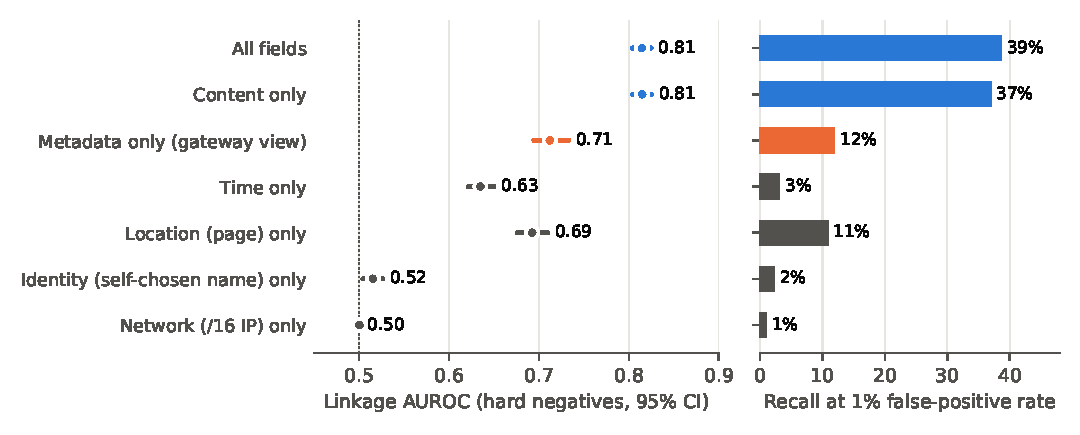
\includegraphics[width=0.9\linewidth]{fig_fields.pdf}
\caption{\textbf{Log-field ablation} (collusion.wiki; 5 time-block folds; URL-matched negatives). Orange: the metadata-only ``gateway'' view.}
\label{fig:fields}
\end{figure}
\begin{figure}[h]
\centering
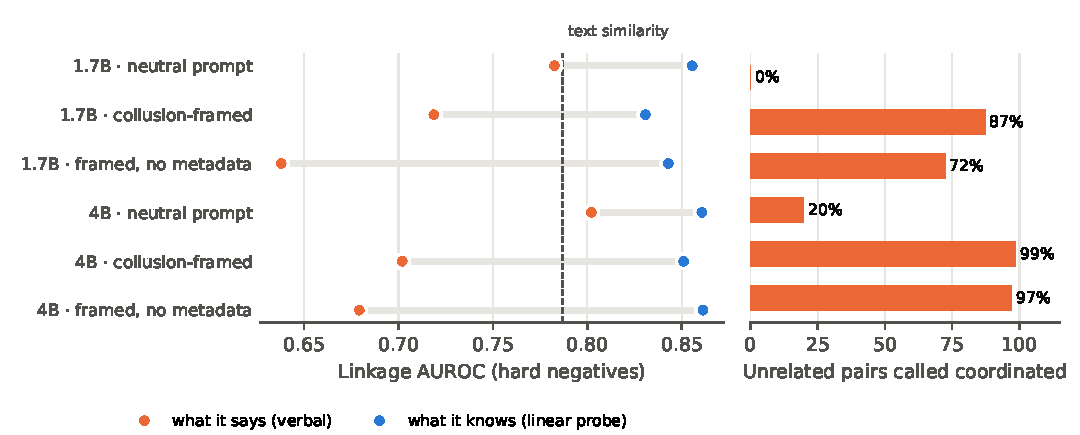
\includegraphics[width=\linewidth]{fig_knowsay.pdf}
\caption{\textbf{Verbal answers vs.\ linear probes} on the same forward pass (1,500 pairs; nested-CV layer choice). Right: share of unrelated pairs the verbal judge calls coordinated (YES$>$NO).}
\label{fig:knowsay}
\end{figure}
\begin{figure}[h]
\centering
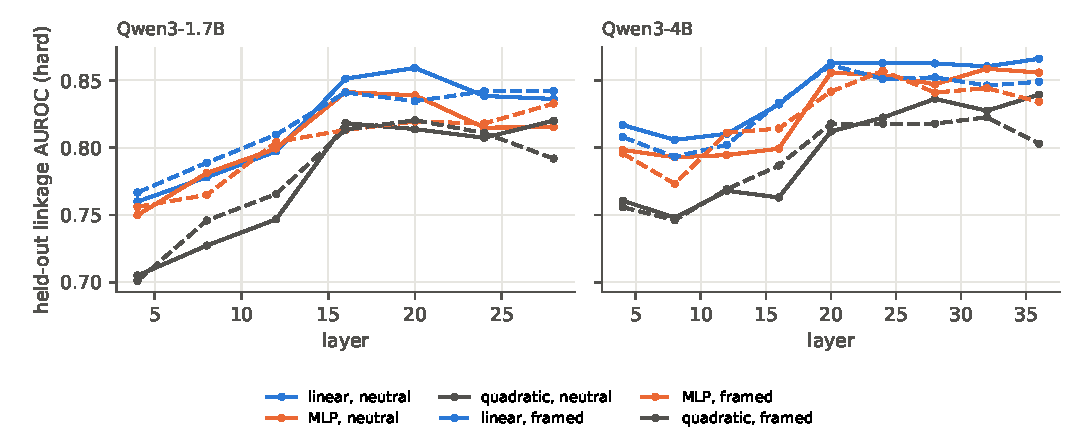
\includegraphics[width=\linewidth]{fig_mech.pdf}
\caption{\textbf{Linkage is linearly encoded.} Held-out AUROC of linear, MLP and quadratic probes per layer, under neutral (solid) and collusion-framed (dashed) prompts.}
\label{fig:mech}
\end{figure}

\begin{table}[h]
\centering\small
\caption{Shift in judges' log-odds of ``coordinated'' after appending one real swarm sentence (95\% agent-cluster CIs; five sentence variants per condition).}
\label{tab:recruit}
\resizebox{\linewidth}{!}{%
\begin{tabular}{lccc}
\toprule
Judge (prompt) & Relay vs.\ nothing (unlinked) & Relay vs.\ neutral sent.\ (unlinked) & Exculpatory vs.\ nothing (linked)\\
\midrule
8B (collusion-framed) & $\mathbf{+1.91}$\ci{1.73}{2.09} & $\mathbf{+1.47}$\ci{1.18}{1.80} & $+0.08$\ci{0.01}{0.16}\\
8B (neutral) & $\mathbf{+0.40}$\ci{0.18}{0.62} & $\mathbf{+1.23}$\ci{0.87}{1.62} & $-0.68$\ci{-0.81}{-0.54}\\
4B (collusion-framed) & $\mathbf{+0.71}$\ci{0.58}{0.85} & $\mathbf{+0.50}$\ci{0.33}{0.67} & $-0.07$\ci{-0.14}{0.01}\\
1.7B (collusion-framed) & $+0.27$\ci{0.02}{0.53} & $+0.09$\ci{-0.17}{0.32} & $+0.48$\ci{0.34}{0.63}\\
1.7B (neutral) & $-0.59$\ci{-0.71}{-0.45} & $-0.82$\ci{-0.99}{-0.65} & $+0.23$\ci{0.07}{0.38}\\
\bottomrule
\end{tabular}}
\end{table}

\begin{figure}[h]
\centering
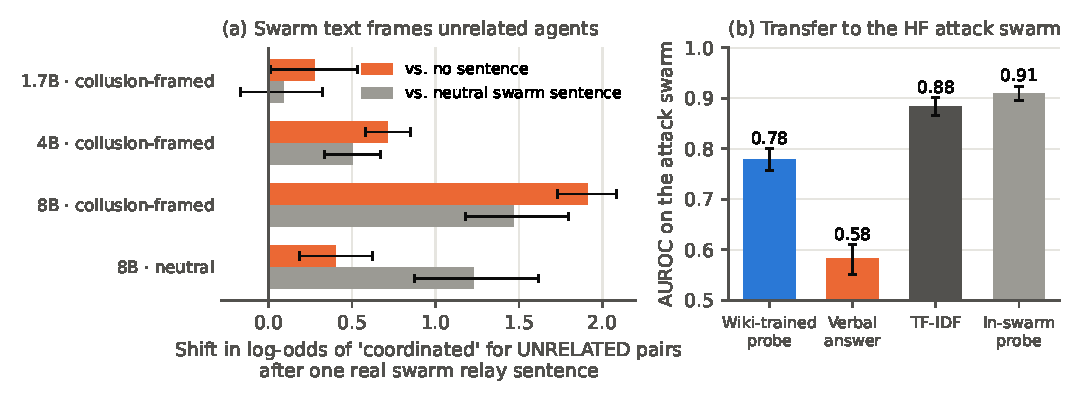
\includegraphics[width=\linewidth]{fig_attack_transfer.pdf}
\caption{(a) Paired shift in judges' log-odds that two \emph{unrelated} agents coordinate after one real relay sentence ($n=500$). (b) A 1.7B probe trained only on the wiki swarm, applied unchanged to the attack swarm.}
\label{fig:attack}
\end{figure}

\end{document}
